\documentclass[sigconf,nonacm]{acmart}
\usepackage{booktabs,tabularx,amsmath,tikz,pgfplots}
\usetikzlibrary{arrows.meta,positioning}
\pgfplotsset{compat=1.18}
\setcopyright{none}
\settopmatter{printacmref=false}
\renewcommand\footnotetextcopyrightpermission[1]{}
\acmConference{}{}{}
\acmYear{2026}
\pagestyle{plain}
\raggedbottom
\setlength{\emergencystretch}{3em}
\Urlmuskip=0mu plus 1mu
\title{When Valid Proofs Do Not Bind the Claimed Statement:\\A Reproduction Study of Five Attestation and SBOM Artifacts}
\author{Ezekiel Ologunde}
\affiliation{\institution{Independent Researcher}\city{Boston}\state{MA}\country{USA}}
\email{ologunde@bu.edu}
\begin{document}
\begin{abstract}
A successful cryptographic verification need not establish the application statement that a consumer intends to accept. We investigate this distinction through a purposive reproduction study of five public software-attestation and software-bill-of-materials (SBOM) artifacts. The study separates witness satisfaction, cryptographic verification, authenticated statement matching, and consumer interpretation. In a PIRANHAS Circom benchmark, changing a response and recomputing its private Merkle root produces a verifying proof while retaining the signature, signature message, and public inputs. The related Noir implementation rejects the tested response mutation. In an archived VeriSBOM command-line verifier, changing auxiliary output metadata makes the application accept an expected root different from the root authenticated by an unchanged Nova proof. A comparator that uses authenticated verifier outputs rejects that mismatch. Selected controls in zRA and TrustBOM reject their specified mutations. zkSBOM correctly rejects changed dependency labels and commitments, while its CLI accepts empty proof files and missing labels under weaker input semantics. We report these as interface behaviors without asserting downstream exploitability. The contribution is an evidence-backed, bounded account of two distinct implementation discrepancies and their diagnostic controls, not a new cryptographic construction, a novel vulnerability class, or a prevalence estimate. Source pins, retained failures, and machine-readable outcomes support review and reproduction.
\end{abstract}
\keywords{zero-knowledge proofs, remote attestation, SBOM, reproducibility, verifier integration}
\maketitle

\section{Introduction}
Public research artifacts make it possible to ask a concrete question: what does an executable verifier actually establish about the statement its caller cares about? Attestation and confidential SBOM sharing are useful settings because a proof commonly sits between a software measurement or inventory and a consumer decision. The decision may depend on an authorized root, a policy, a device identity, or a query. A verifier returning success is only one part of that chain.

We examine five artifacts associated with zRA, PIRANHAS, TrustBOM, zkSBOM, and VeriSBOM~\cite{zra,piranhas,trustbom,zksbom,verisbom}. We do not compare their performance as interchangeable implementations. They use different statements, proof systems, trust anchors, and workloads. Instead, we reconstruct selected local execution paths and make controlled changes at explicit boundaries. A positive proof is required before a rejection is interpreted. We distinguish rejection during witness generation from rejection of a completed proof, and both from rejection by an application comparator.

Two results motivate the study. First, the tested PIRANHAS Circom benchmark enforces a Merkle relation and a signature relation without requiring the signature message to authenticate the root used by the former. Second, the archived VeriSBOM CLI checks proof validity but compares caller expectations to separately deserialized metadata rather than the final outputs authenticated by verification. Both results concern the pinned executable paths. Neither demonstrates a failure of the underlying proof system or an attack on a complete deployed protocol.

This paper contributes (1) reproducible evidence for those two discrepancies, including field-isolated controls; (2) diagnostic comparisons with a modified relation or authenticated-output consumer; and (3) an explicit account of correctly rejecting controls, interface ambiguities, and reproduction failures across the selected corpus. The organizing ledger is a reporting device, not a claimed new detector. The study was exploratory: its common protocol was consolidated after initial findings. It is not a preregistered discovery experiment or an independently evaluated benchmark.

\section{Background and Related Work}
A proof verifier checks a relation under a particular verification key or program identifier. An application must additionally establish that the authenticated values correspond to its intended context. In one implementation, this requires exposing the right public inputs. In another, verification returns authenticated outputs that must be used by the caller. A serialized bundle can also contain descriptive values that are not authenticated merely because they travel with a valid proof.

Layered ZKP auditing is established practice. Tang et al. describe analysis from application design through primitive integration~\cite{audit}. Our separation of proof validity and application meaning therefore does not introduce a new audit principle. Picus checks uniqueness properties of circuit signals~\cite{picus}; Circomspect provides Circom-specific static analysis~\cite{circomspect}. zkFuzz formulates trace--constraint consistency and tests circuits through program mutation~\cite{zkfuzz}. These approaches address important properties, but their stated circuit targets are not equivalent to arbitrary Rust consumer logic. An unsupported target is not a measured analyzer failure.

The study artifacts span different applications. zRA concerns transparent non-interactive attestation, and PIRANHAS extends privacy-preserving attestation to swarms~\cite{zra,piranhas}. TrustBOM, zkSBOM, and VeriSBOM concern confidential or selectively disclosed SBOM properties~\cite{trustbom,zksbom,verisbom}. We use their public artifacts as executable case studies rather than claiming that the complete protocols share one security definition. Our observations are specifically attributed to backend, revision, fixture, and consumer path.

The empirical distinction from these systems' original evaluations is the controlled comparison of accepted statements with application expectations. That distinction is a scope description, not a priority claim. We have not established that the two observed artifact discrepancies were previously unknown, and no independent novelty assessment or author confirmation has been obtained. The targeted literature screen also does not establish systematic-review completeness.

\section{Study Design}
\subsection{Questions and units of analysis}
We ask three questions. RQ1: which selected mutations preserve cryptographic verification while violating an intended connection between statement components? RQ2: do diagnostic controls remove the observed acceptance without treating every changed input as invalid? RQ3: what distinctions must a consumer retain when interpreting proof validity, query identity, and membership?

The unit of analysis is a pinned artifact execution path. A Circom and a Noir backend from the same artifact are not independent systems. The five-system corpus was selected purposively for relevance and feasible public evidence, after pilot observations. zRA and PIRANHAS share intellectual lineage, and VeriSBOM shares an author with that line. We therefore report no defect percentage, confidence interval, or population prevalence. Cases are fixed counterexamples and controls, not independent random trials.

\subsection{Statement ledger}
For each case we record an expected value and its origin, the witness relation, the authenticated public input or output, the consumer comparison, and the final decision. An unsupported application expectation is marked outside the demonstrated contract. The ledger is intentionally conservative: absence of an observed check is a lead; a completed proof with a demonstrated mismatch is stronger evidence; a deployed exploit would require further caller and threat-model evidence.

Let $\pi$ be a proof, $x$ its authenticated statement, $m$ auxiliary bundle metadata, and $e$ a caller expectation. Write $V(\pi)=x$ for successful verification that returns outputs; for public-input systems, read $V(\pi,x)=1$ instead. A consumer obligation is a predicate $B(x,e)$. A bundle-level test can expose a mismatch when
\begin{equation}
 V(\pi)=x,\qquad A(\pi,m,e)=1,\qquad B(x,e)=0.
\end{equation}
This notation is a bookkeeping model, not a security theorem. The trustworthiness and completeness of $e$ must be justified separately. For an internal circuit disconnect, the relevant obligation links two witness-derived terms; no external equality test can repair a missing relation merely by trusting another unauthenticated field.

\subsection{Controls and decision rules}
We require an honest positive case, then change one logical condition at a time. Where possible, we retain the exact serialized proof and vary expected values or auxiliary metadata. When a witness must change, we record the changed fields and regenerate a real proof against the same relation. We retain failed attempts and do not count environment errors as cryptographic rejections.

A useful diagnostic control must preserve correct acceptance as well as reject mismatches. For example, changing ignored redundant metadata is harmless if the consumer uses the authenticated output and that output matches its expectation. Rejecting every metadata edit would conceal this distinction. We also include correctly bound implementations and record failure stage: witness, proof verifier, application comparison, or execution failure.

\subsection{Corpus and environment}
Table~\ref{tab:corpus} records the executed scope. Repository revisions are included in the accompanying ledger and summarized in Appendix~\ref{sec:repro}. Experiments ran locally in bounded Linux Docker containers on a Windows host; no HPC job or external service test was involved. Tool versions, image identifiers, source hashes, and commands are preserved. Resource changes in an earlier TrustBOM run and heterogeneous builds make elapsed times unsuitable for a comparative benchmark.

\begin{table*}[t]
\caption{Executed scope and principal limits. Passing selected controls is not comprehensive security assurance.}
\label{tab:corpus}
\small
\begin{tabularx}{\textwidth}{@{}lXX@{}}
\toprule Artifact & Executed evidence & Excluded or unresolved scope \\
\midrule
zRA & Fresh proof with shipped depth-40 WASM/key; public root, address and challenge controls & Source-to-binary correspondence and on-chain caller execution \\
PIRANHAS & Circom proof mutation; Noir proof and witness controls; local alternative relation & Full swarm protocol; Plonky2 execution; repair equivalence \\
TrustBOM & Non-Fake RISC Zero receipt; saved-receipt consumer controls & HTTP deployment, full operational stack and policy generality \\
zkSBOM & Default oZKS native wrapper and original Rust CLI controls & Operator/advisory service; upstream unit tests did not pass \\
VeriSBOM & Archived source-built Nova CLI; unchanged-proof metadata controls & Hosted service; fresh circuit/parameter derivation; depositor identity \\
\bottomrule
\end{tabularx}
\end{table*}

\section{PIRANHAS: Separately Satisfied Relations}
\subsection{Observed benchmark behavior}
At the pinned revision, the Circom benchmark supplies a private root to its Merkle component and a separate message to its Schnorr component. The public vector contains enabled, pubX, and pubY. We first reproduced an honest witness and proof. We then increased the response by one. Retaining the old root failed witness generation; recomputing the root restored the Merkle relation. With the original signature and message unchanged, the new witness satisfied the unchanged R1CS and produced a verifying Groth16 proof. Both accepted proofs exposed the same public vector.

The result distinguishes two enforced properties from their missing connection. The old-root mutation confirms that the Merkle equation is active. A changed signature scalar fails its witness assertion, confirming that the tested signature equation is active. The jointly changed response and root demonstrate that satisfying both equations does not itself bind them together. This is an implementation-to-intended-relation discrepancy in a benchmark path, not a signature forgery.

The related Noir implementation derives the signed message from the root and key. Its honest fixture solved and yielded a verifying UltraHonk proof. The tested response mutation and signature-byte mutation failed at the signature assertion. A serialization-preserving public-key mutation of a saved proof was explicitly rejected. An earlier first-byte proof corruption terminated with exit 139; we retain that event as abnormal termination rather than presenting it as a clean verifier rejection. The backends differ in their public interfaces, so these results do not establish semantic equivalence or a performance ranking.

\subsection{Diagnostic alternative relation}
A researcher-defined Circom relation derives its signed message internally and adds domain-separated Poseidon encodings for the leaf, message, and tag. It makes challenge and tag public, constrains enabled to one, and removes the device-address leaf field. These are substantive relation changes. The construction is therefore an alternative diagnostic instantiation, not a certified patch implementing the paper's exact relation.

The positive fixture produced a real verifying proof. Six negative witness cases were rejected: changed response with stale root; changed response with recomputed root and old signature; changed secret key; changed tag; changed challenge; and changed signature scalar. Separately, altering the public challenge of the saved positive proof caused verifier rejection. The test signer and nonce were deterministic and public for fixture construction, unsuitable for deployment.

Figure~\ref{fig:size} reports compiled constraint counts from the two local relations. The increase is a size observation only: the relation, public interface, and checks changed. It is not an efficiency comparison with Noir or a runtime overhead estimate.

\begin{figure}[t]
\centering
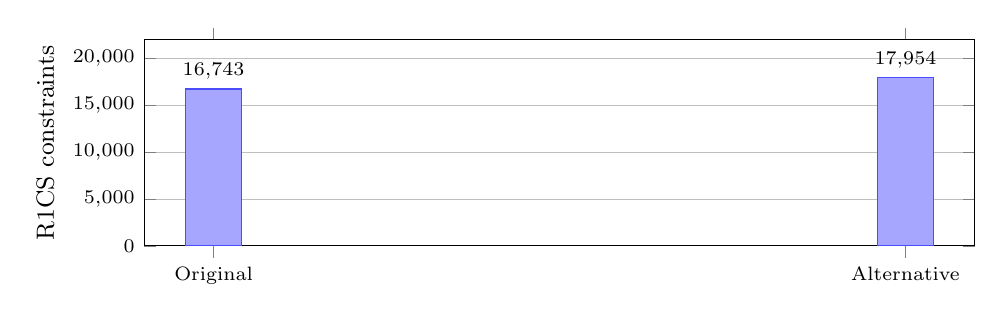
\begin{tikzpicture}
\begin{axis}[ybar,bar width=20pt,width=\columnwidth,height=4.2cm,ymin=0,ymax=22000,ylabel={R1CS constraints},symbolic x coords={Original,Alternative},xtick=data,nodes near coords,nodes near coords style={font=\scriptsize},tick label style={font=\scriptsize},label style={font=\small},scaled y ticks=false,ytick={0,5000,10000,15000,20000},ymajorgrids=true]
\addplot[fill=blue!35,draw=blue!70] coordinates {(Original,16743) (Alternative,17954)};
\end{axis}
\end{tikzpicture}
\caption{Local Circom size comparison: 16,743 versus 17,954 constraints, an increase of 1,211 (7.23\%). The alternative changes the relation; this is not runtime overhead.}
\Description{Two bars show 16743 original constraints and 17954 alternative constraints.}
\label{fig:size}
\end{figure}

\subsection{Analyzer interpretation}
Circomspect at a pinned revision reported two informational categories for each selected top-level Circom file. The compiler inspection pass also produced component-signal warnings. Neither output explicitly diagnosed the root/signature contract in these runs. Equal warning counts do not mean equal semantics, and these observations do not establish a false-negative rate. We did not execute Picus or zkFuzz on the artifacts. An ordinary manual inspection of the relation can identify the disconnect, so this experiment cannot justify superiority of a new automated detector.

\section{VeriSBOM: Unauthenticated Output Metadata}
\subsection{Fixture and authenticated outputs}
We acquired the archive associated with Zenodo record 21372814~\cite{veriartifact}, checked its recorded archive checksum, and retained source hashes. The depositor uses the alias VeriSBOM; individual depositor identity was not independently authenticated. The local test uses the archived CLI, not its hosted application.

The honest fixture contains one authorized package in the archived depth-10 circuit. Expected package-manager and auditor roots were created before proof generation using the archived helpers. The authorization policy is explicitly synthetic. These checks establish fixture consistency, not independent correctness of the hash helpers, real-world package policy, or SBOM completeness. The Rust prover/verifier was built from archived source with its lockfile; circuit files and public parameters were taken from the archive.

The verifier calls Nova verification and checks success. It then reads the separate bundle vector \texttt{zi\_primary} to compare the expected SBOM hash, package-manager root, and auditor root. The authenticated primary outputs returned by successful verification are not used for those comparisons. A probe confirmed that the honest auxiliary vector initially agreed with the authenticated output. It incremented only the auxiliary package-manager-root field by one and reverified the proof. The authenticated output and the serialized cryptographic proof core remained unchanged.

\subsection{Paired acceptance experiment}
Table~\ref{tab:veri} shows four bundle/expectation combinations for the unchanged CLI and a diagnostic comparator. All eight executions passed cryptographic verification. Changing only the expected root makes the original CLI reject; changing only auxiliary metadata also makes it reject. Changing both causes it to accept even though the proof authenticates the original root. No cryptographic proof was forged or regenerated for this discrepancy.

\begin{table}[t]
\caption{VeriSBOM decisions. All rows use a mathematically valid proof. The diagnostic comparator uses authenticated outputs.}
\label{tab:veri}
\centering\small
\begin{tabular}{@{}llll@{}}
\toprule Metadata & Expected root & Archived & Diagnostic \\
\midrule
Original & Original & Accept & Accept \\
Original & Changed & Reject & Reject \\
Changed & Original & Reject & Accept \\
Changed & Changed & Accept & Reject \\
\bottomrule
\end{tabular}
\end{table}

The diagnostic comparator uses Nova's authenticated primary output for the three value comparisons and length checks. It rejects both cases with the changed expected root. It accepts the metadata-only case because the authenticated root still matches the original expectation. This is the intended positive control: unused auxiliary data does not change the proven statement. Figure~\ref{fig:flow} illustrates the observed consumer paths.

\begin{figure}[t]
\centering
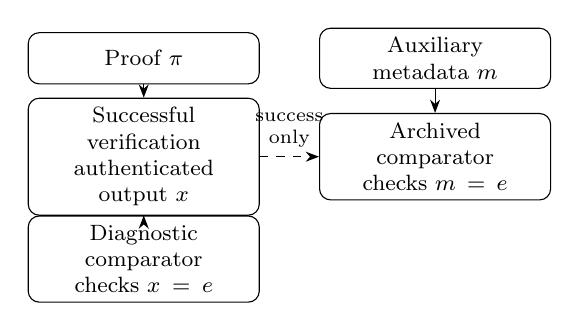
\begin{tikzpicture}[font=\footnotesize,box/.style={draw,rounded corners,align=center,text width=2.7cm,minimum height=.65cm},>=Stealth]
\node[box] (proof) at (0,0) {Proof $\pi$};
\node[box] (meta) at (3.7,0) {Auxiliary metadata $m$};
\node[box] (auth) at (0,-1.25) {Successful verification\\authenticated output $x$};
\node[box] (old) at (3.7,-1.25) {Archived comparator\\checks $m=e$};
\node[box] (fixed) at (0,-2.55) {Diagnostic comparator\\checks $x=e$};
\draw[->] (proof)--(auth);
\draw[->] (meta)--(old);
\draw[->] (auth)--(fixed);
\draw[->,dashed] (auth)--node[above,font=\scriptsize,align=center]{success\\only}(old);
\end{tikzpicture}
\caption{VeriSBOM's tested data flow. The archived path gates on proof success but compares auxiliary values; the diagnostic path compares authenticated outputs. Arrows denote dependencies, not a measured causal model.}
\Description{The proof feeds verification and authenticated output x. The original comparator receives success and separate metadata m. The diagnostic comparator compares x with the expected value e.}
\label{fig:flow}
\end{figure}

The required threat condition is an untrusted bundle supplied to this CLI with an independently chosen expected root. The caller does not have to alter its expectation maliciously: the two roots are alternative fixed test contexts. What remains untested is whether a deployment restricts bundle provenance or adds a check outside this path. We consequently attribute the finding to the archived local verifier and do not claim a hosted exploit or a Nova soundness failure.

\section{Controls and Consumer Semantics}
\subsection{zRA and TrustBOM}
The zRA reproduction generated a fresh witness and proof using the shipped depth-40 WASM and key. Mutating the public root, device address, or challenge separately caused rejection. A changed response with the old root and path failed witness generation. Source inspection identifies authorization and challenge checks in the Solidity caller, but that contract was not executed. The results cover the shipped artifacts, not independently established source-to-binary correspondence or setup trust.

For TrustBOM, a real RISC Zero receipt was generated for a two-entry public fixture with developer mode disabled and Fake receipts excluded. The expected program identifier, root, policy digest, and compliance output were checked. Wrong program identifier and altered journal controls rejected. A subsequent local adapter exercised six saved-receipt controls, including expected-context comparisons. This is evidence for the tested guest/consumer path, not for an HTTP service or the full operational deployment. Neither system is classified as secure merely because its selected controls passed.

\subsection{zkSBOM: validity is not a query answer}
The default oZKS backend was built without replacing it with an ordinary Merkle mode. The unchanged C++ wrapper returned valid-member and valid-nonmember codes for genuine proofs and rejected a previous member proof against a changed commitment. Extracted keys matched. Three wrapper controls were repeated with independently constructed dependency-hash keys. The original Rust application source and wrapper were then built using a documented link-only adapter.

Table~\ref{tab:zksbom} reports the six CLI cases. A wrong dependency label and changed commitment produced invalid messages. Missing labels skip key-to-label binding, and an empty proof file reaches a vacuously true aggregate result. Every tested case exited with code zero, including invalid messages. A caller relying only on the process exit code would therefore lose a distinction visible in the CLI output.

\begin{table}[t]
\caption{zkSBOM CLI output. A valid message is not sufficient to establish an answer to a caller-specified nonempty query.}
\label{tab:zksbom}
\centering\small
\begin{tabular}{@{}lll@{}}
\toprule Case & Validity message & Exit code \\
\midrule
Honest member & Valid & 0 \\
Honest nonmember & Valid & 0 \\
Wrong label & Invalid & 0 \\
Missing label & Valid & 0 \\
Changed commitment & Invalid & 0 \\
Empty file & Valid & 0 \\
\bottomrule
\end{tabular}
\end{table}

We applied an ordinary output-level consumer predicate to the saved results: require an overall valid message, exactly one nonempty dependency equal to the independently expected query, and an explicit member/nonmember answer. It accepts both honest answer types and rejects the remaining cases. This is not another cryptographic verification and not a new algorithm. The wrong-label case can still print a membership detail alongside an overall invalid result; the aggregate decision must take precedence.

These observations do not establish an exploitable third vulnerability. A low-level verifier may legitimately report proof validity without enforcing a downstream requirement for a nonempty expected query. We did not execute a deployed caller that promises and then violates that requirement. The result is a reproducible warning about interface interpretation, clearly separated from the two demonstrated relation/output discrepancies.

\section{Evidence Integrity and Reproduction}
Evidence directories retain commands, image identifiers, source pins, file hashes, exit codes, and logs. Verification scripts independently parse the saved outputs and compare frozen file hashes; they do not independently reimplement Nova, Groth16, UltraHonk, RISC Zero, or oZKS. Byte identity is a particularly useful invariant in the VeriSBOM case because it rules out a changed cryptographic proof as the source of changed application acceptance.

The study also retains unsuccessful runs. An initial local Circom setup lacked contributions and failed a public-key control; it was excluded and replaced by an explicitly amended setup. Noir required environment packages before proof generation. The malformed-proof exit 139 remains visible. VeriSBOM required a compatible C++ runtime and a corrected driver filename after successful proof production. zkSBOM required a Flatbuffers package-name shim and explicit linking of archived Blake2 code for its wrapper probe. Distributed tests failed compilation, and upstream simple tests did not link successfully. Those tests are not reported as passed. The Rust CLI's build script was replaced only to link the existing native library and distro dependencies; application code remained unchanged.

The main numeric observations and decision tables are generated from machine-readable records and checked independently against their evidence snapshots. Hash-check counts describe bookkeeping operations, not independent scientific samples. Generated keys, raw proof bundles, third-party source archives, and downloaded papers are excluded from the manuscript package. The repository records acquisition and reproduction instructions; a fresh proof reproduction still requires those external inputs and local build steps. Rebuilding the paper is a separate and much smaller operation.

\section{Discussion and Threats to Validity}
\subsection{What the observations support}
The two discrepancies have different locations. In the PIRANHAS benchmark, the missing connection is inside the implemented relation: two individually satisfied subrelations do not establish their intended linkage. In VeriSBOM, cryptographic verification authenticates an output, but the consumer compares another representation. A common symptom, successful verification, does not make these the same defect or imply a shared repair.

The diagnostic controls are correspondingly different. An alternative circuit relation can connect the signed message to the root, but requires new proof generation and changes semantics. A consumer can instead use already authenticated outputs without altering a proof. Treating both cases as generic input tampering would hide that distinction. Correctly rejecting cases in the corpus and the harmless metadata-only repair case limit overbroad interpretations.

\subsection{Internal and construct validity}
The audit was conducted with source access and knowledge of initial results. Case selection and diagnostic repairs are not blinded. Fixture construction and verification share upstream cryptographic libraries, so independent evidence parsing does not eliminate common implementation errors. The public deterministic signer used by the candidate circuit is only a test fixture. Archived parameter and shipped-binary provenance are not equivalent to a production trust establishment process.

Application obligations are another source of uncertainty. A benchmark simplification may explain an implementation difference without invalidating a paper's formal construction. Empty-input acceptance may be permitted by a low-level API and rejected by a higher layer. We avoid converting those possibilities into either blanket exoneration or unsupported exploit claims. The paper reports the exact tested boundary and leaves unexecuted callers unresolved.

\subsection{External validity and novelty}
The sample is small, purposive, and partly related by authorship and research lineage. Backend executions and repeated controls are not additional systems. Workloads are deliberately small, and neither scaling nor operational resilience was evaluated. No prevalence or comparative performance estimate follows.

Known application-binding principles explain the observations. The study does not establish a new vulnerability class, first discovery, or tool superiority. Its potential value is the inspectable empirical record: executable counterexamples, contrasting implementations, diagnostic controls, and retained failures. Whether that bounded contribution meets a particular journal's novelty threshold remains an editorial and peer-review question, not an experimental result.

\subsection{Ethics, disclosure, and assistance}
All executions were local and used public research artifacts and synthetic or public fixtures. No hosted system, third-party account, or live organizational inventory was tested. No issue filing, author contact, or journal submission has occurred. The absence of maintainer confirmation limits interpretation of intended artifact scope. Public reports are restricted to the local evidence and do not describe operational exploitation. No funding or institutional affiliation is inferred. AI-assisted tools supported coding, literature screening, analysis, and manuscript preparation; the named author must review the manuscript and its claims before submission.

\section{Conclusion}
In five selected artifacts, proof execution and application interpretation required separate examination. We reproduced a benchmark relation disconnect in PIRANHAS and an authenticated-output comparison discrepancy in an archived VeriSBOM CLI. Diagnostic controls removed the tested acceptances, with different implications for relation semantics. zRA and TrustBOM passed selected controls; zkSBOM exposed consumer-interface boundaries without establishing downstream exploitability. These findings support a bounded empirical reproduction paper. They do not prove a new cryptographic method, representative defect prevalence, or prior-art novelty.

\begin{thebibliography}{10}
\sloppy
\bibitem{zra} Shahriar Ebrahimi and Parisa Hassanizadeh. 2024. From Interaction to Independence: zkSNARKs for Transparent and Non-Interactive Remote Attestation. NDSS. \url{https://www.ndss-symposium.org/wp-content/uploads/2024-815-paper.pdf}
\bibitem{piranhas} Jonas Hofmann, Philipp-Florens Lehwalder, Shahriar Ebrahimi, Parisa Hassanizadeh, and Sebastian Faust. 2026. PIRANHAS: PrIvacy-Preserving Remote Attestation in Non-Hierarchical Asynchronous Swarms. NDSS. \url{https://www.ndss-symposium.org/wp-content/uploads/2026-f526-paper.pdf}
\bibitem{trustbom} Van Thang Nguyen et al. 2026. TrustBOM: A Scalable Architecture for Confidentiality-Preserving SBOMs Across Organizations. arXiv:2609.21419v1. \url{https://arxiv.org/abs/2609.21419v1}
\bibitem{zksbom} Tom Sorger, Eric Cornelissen, Aman Sharma, Javier Ron, Musard Balliu, and Martin Monperrus. 2026. zkSBOM: Privacy-Preserving SBOM Sharing with Zero-Knowledge Sets. arXiv:2605.00076v1. \url{https://arxiv.org/abs/2605.00076v1}
\bibitem{verisbom} Gianpietro Castiglione, Shahriar Ebrahimi, and Narges Khakpour. 2026. VeriSBOM: Secure and Verifiable SBOM Sharing Via Zero-Knowledge Proofs. arXiv:2602.13682v1. \url{https://arxiv.org/abs/2602.13682v1}
\bibitem{veriartifact} VeriSBOM. VeriSBOM Artifact. Zenodo record 21372814. Accessed October 8, 2026. \url{https://zenodo.org/records/21372814}
\bibitem{audit} Xueyan Tang, Lingzhi Shi, Xun Wang, Kyle Charbonnet, Shixiang Tang, and Shixiao Sun. 2024. Zero-Knowledge Proof Vulnerability Analysis and Security Auditing. Cryptology ePrint Archive, 2024/514. \url{https://eprint.iacr.org/2024/514}
\bibitem{picus} Veridise. Picus: Automated verification of uniqueness property for ZKP circuits. Accessed October 8, 2026. \url{https://github.com/Veridise/Picus}
\bibitem{circomspect} Trail of Bits. Circomspect: A static analyzer and linter for the Circom zero-knowledge DSL. Accessed October 8, 2026. \url{https://github.com/trailofbits/circomspect}
\bibitem{zkfuzz} Hideaki Takahashi, Jihwan Kim, Suman Jana, and Junfeng Yang. 2026. zkFuzz: Foundation and Framework for Effective Fuzzing of Zero-Knowledge Circuits. IEEE Symposium on Security and Privacy. \url{https://www.cs.columbia.edu/~junfeng/papers/zkfuzz/}
\end{thebibliography}

\appendix
\section{Artifact Identification and Review Guide}\label{sec:repro}
The evidence repository is \url{https://github.com/ezekielologunde/zkp-remediation-assurance}. The input evidence snapshot for this manuscript follows commit \texttt{70a6f01}; the package contains hashes identifying the precise copied records. Original research remains unlicensed; third-party material retains its own terms. The manuscript package does not grant additional rights to third-party code or datasets.

The selected source pins are zRA \texttt{4a0416c}, PIRANHAS \texttt{62bd2af}, TrustBOM \texttt{ea90058}, and zkSBOM \texttt{0bb63ac}, with oZKS \texttt{5a7d43d}. VeriSBOM is identified by Zenodo record 21372814 and the archive checksum in the repository ledger. Full revisions and source manifests are retained there rather than relying on these abbreviated identifiers.

For PIRANHAS, begin with the root-binding and backend-comparison verification records, then the repair and analyzer records. For VeriSBOM, compare the acceptance and repair case JSON files with their logs and the bundle-probe receipt. For zkSBOM, inspect the six CLI logs before interpreting the aggregate verifier message. The manuscript ZIP includes a lightweight table/figure verifier and its supporting evidence snapshots. It validates the paper's presentation of saved results, not fresh cryptographic execution or third-party source correctness.
\end{document}
